\documentclass[xcolor=dvipsnames]{beamer}
\usecolortheme[named=MidnightBlue]{structure}
\definecolor{blue(ryb)}{rgb}{0.2, 0.2, 0.6}
\definecolor{blue(ryb)}{rgb}{0.01, 0.28, 1.0}
\definecolor{bostonuniversityred}{rgb}{0.8, 0.0, 0.0}
\DeclareGraphicsExtensions{jpg,eps,png}
 \renewcommand{\thefootnote}{\fnsymbol{footnote}}
\usetheme{Boadilla} 
%--------------modify footer
\makeatother
\setbeamertemplate{footline}
{
  \leavevmode%
  \hbox{%
   \begin{beamercolorbox}[wd=.4\paperwidth,ht=2.25ex,dp=1ex,center]{section in head/foot}%
    \usebeamerfont{section in head/foot}\insertsectionhead
  \end{beamercolorbox}%
  \begin{beamercolorbox}[wd=.6\paperwidth,ht=2.25ex,dp=1ex,center]{title in head/foot}%
    \usebeamerfont{section in head/foot}\insertshorttitle\hspace*{3em}
    \insertframenumber{} / \inserttotalframenumber\hspace*{1ex}
  \end{beamercolorbox}}%
  \vskip0pt%
}
\makeatletter
\setbeamertemplate{navigation symbols}{}
%---------------------------modify footer end
\usepackage[absolute,overlay]{textpos}
\newcommand\hypercorner[1]{%
  \begin{textblock*}{\paperwidth}(0pt,255pt)
    \raggedleft #1\hspace{.5em}
  \end{textblock*}}
  
%\hypersetup{pdfpagemode=FullScreen}
\usepackage{epsfig}
\usepackage{graphicx}
\usepackage{epstopdf}
\graphicspath{{Figures/}}

\newcommand\hyperback[1]{%
  \begin{textblock*}{\paperwidth}(10pt,254pt)
    \raggedright #1\hspace{.5em}
  \end{textblock*}}
  
%\hypersetup{pdfpagemode=FullScreen}
\usepackage{epsfig}
\usepackage{graphicx}
\usepackage{epstopdf}
\graphicspath{{Figures/}}
%-------------------------------------
%Title
%-------------------------------------

\title[]{Communication Efficient Data Exchange Among Multiple Nodes}
\author[]{Soumya Subhra Banerjee \\\vspace{.5cm} \tiny \textit{Under guidance of,}\\\normalsize Himanshu Tyagi }
\normalsize
\institute[ECE, IISc]{Mid-Term Project presentation,\\ EP 299 Project, M.Tech, Communication and Networks, ECE}
\date{\today}
%====================================Title
\begin{document}
\begin{frame}
\titlepage
\end{frame}
%====================================Overview

\section{Overview}

%-------------------motivation
\begin{frame}[label = motivation]
\frametitle{Motivation}
\framesubtitle{The Data-Exchange problem}
\begin{figure}[!htb]
\begin{center}
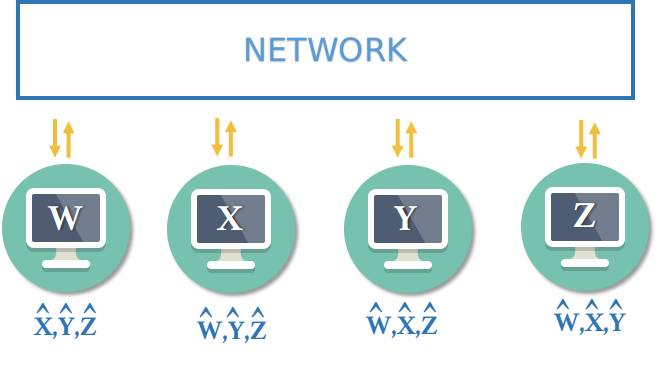
\includegraphics[scale=0.4]{./multipartydataex.png}
\label{fig:exitfun}
\end{center}
\end{figure}
Multiple parties observing correlated data seek to recover each other's data. How can they accomplish this using minimum communication?
\end{frame}

%-------------------Two party case
\begin{frame}[label = twoparty]
\frametitle{The Data-Exchange Problem}
\framesubtitle{Two party case}
\begin{minipage}[0.9\textheight]{\textwidth}
\begin{columns}
\begin{column}{0.4\textwidth}
\begin{itemize}
\item Random correlated data (X,Y) is distributed between two parties.
\item The first observes X and second observes Y.
\item They seek to recover each others data.
\item The joint distribution of X and Y is unknown.
\end{itemize}
\end{column}
\begin{column}{0.5\textwidth}
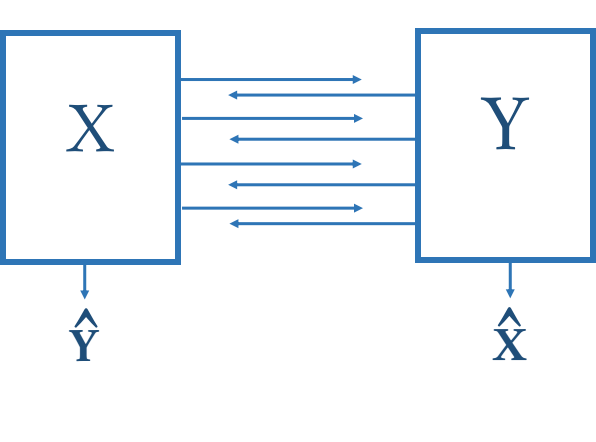
\includegraphics[width=5.2cm]{./dataexp.png}
\end{column}
\end{columns}
\end{minipage}\\
\vspace{0.5cm}
This project seeks to device a protocol which achieves this with minimal communication. 
\end{frame}

%----------------------rsynccomp
\begin{frame}[label= rsynccomp]
\frametitle{Working Solution}
\framesubtitle{r-sync vs Slepian-Wolf compression}
\begin{itemize}
\item In practice, algorithms like r-sync are used for data exchange.
\begin{itemize}
\item Uses \emph{one} guess.
\item Does not exploit the correlation between the data well.
\item Needs more communication.
\item Fast and low complexity.
\end{itemize}
\end{itemize}
\begin{minipage}[0.5\textheight]{\textwidth}
\begin{columns}
\begin{column}{0.4\textwidth}
\begin{itemize}
\item In theory, Slepian-Wolf compression is optimal. 
\begin{itemize}
\item Under joint decoding $H(X|Y)$ is sufficient to estimate X.
\end{itemize}
\end{itemize}
\end{column}
\begin{column}{0.5\textwidth}
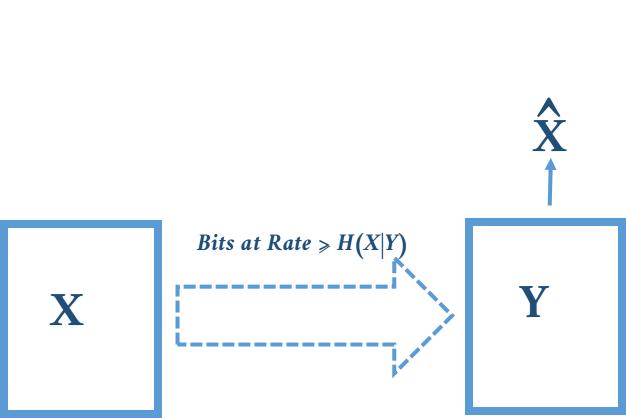
\includegraphics[width=5.2cm]{./swcompp.png}
\end{column}
\end{columns}
\end{minipage}
\hypercorner{\hyperlink{rsync}{\beamerbutton{r-sync}}}
\end{frame}

%--------------------implementation of slepian wolf
\begin{frame}
\frametitle{Implementation of SW compression.}
\framesubtitle{ Difficulties and suggested approach...}
Difficulties in implementaion of SW compression
\begin{itemize}
\item Search is over an exponential list in decoding.
\item Knowledge of $P_{X|Y}$ is required at encoder.
\end{itemize}
\begin{block}{Suggested Approach}
\begin{itemize}
\item{Implement SW Compression using Polar Codes.}
\item{Achieve universality using \emph{recursive data exchange} protocol (RDE).}
\item{Realise RDE using Rateless Polar Codes with physical layer error detection.}
\end{itemize}
\end{block}
\end{frame}

%===========================Outline
\section{Outline}
\begin{frame}
\frametitle{Outline}
\begin{itemize}
\item Background
\begin{itemize}
\item{Recursive Data Exchange (RDE)}
\item{Brief introduction to Polar Codes}
\item{Slepian-Wolf compression with Polar Codes}
\item{Rateless Polar Codes}
\end{itemize}
\item Proposed implementation of RDE
\begin{itemize}
\item Adaptation of Rateless Polar Code for RDE
\item PHY-Layer error detection
\end{itemize}
\item Performance evaluation
\item Conclusion and future work
\end{itemize}
\end{frame}

%============================background
\section{Background}

%----------------------------RDE
\begin{frame}[label = rde]
\frametitle{Recursive Data Exchange (RDE)}
The \emph{recursive data exchange}\footnote{\tiny H. Tyagi and S. Watanabe, Universal Multiparty Data Exchange and Secret Key arrangement, \textit{ISIT,} 2016} protocol is based on an interactive version of the SW protocol 
\begin{itemize}
\item Here the length of communication is increased in steps until the second party decodes the data of the first.
\item After each transmission second party sends ACK-NACK feedback signal, the protocol stops when ACK is recieved or some fixed number of bits have been transmitted.
\item This protocol is \emph{universal} as it does not rely on knowledge of the joint distribution.
\item It uses an iterative variable length approach to reach rate optimality universally. 
\item The suggested decoders are theoritical constructs which use type classes to form a list of guesses for data of other parties and thus has exponential complexity.
\end{itemize}
\end{frame}

%----------------------------Polar codes
\begin{frame}[label = polarcodes]
\frametitle{Brief Introduction to Polar Codes}
\framesubtitle{Channel polarization}
\begin{minipage}[0.9\textheight]{\textwidth}
\begin{columns}
\begin{column}{0.6\textwidth}
\begin{figure}
\centering
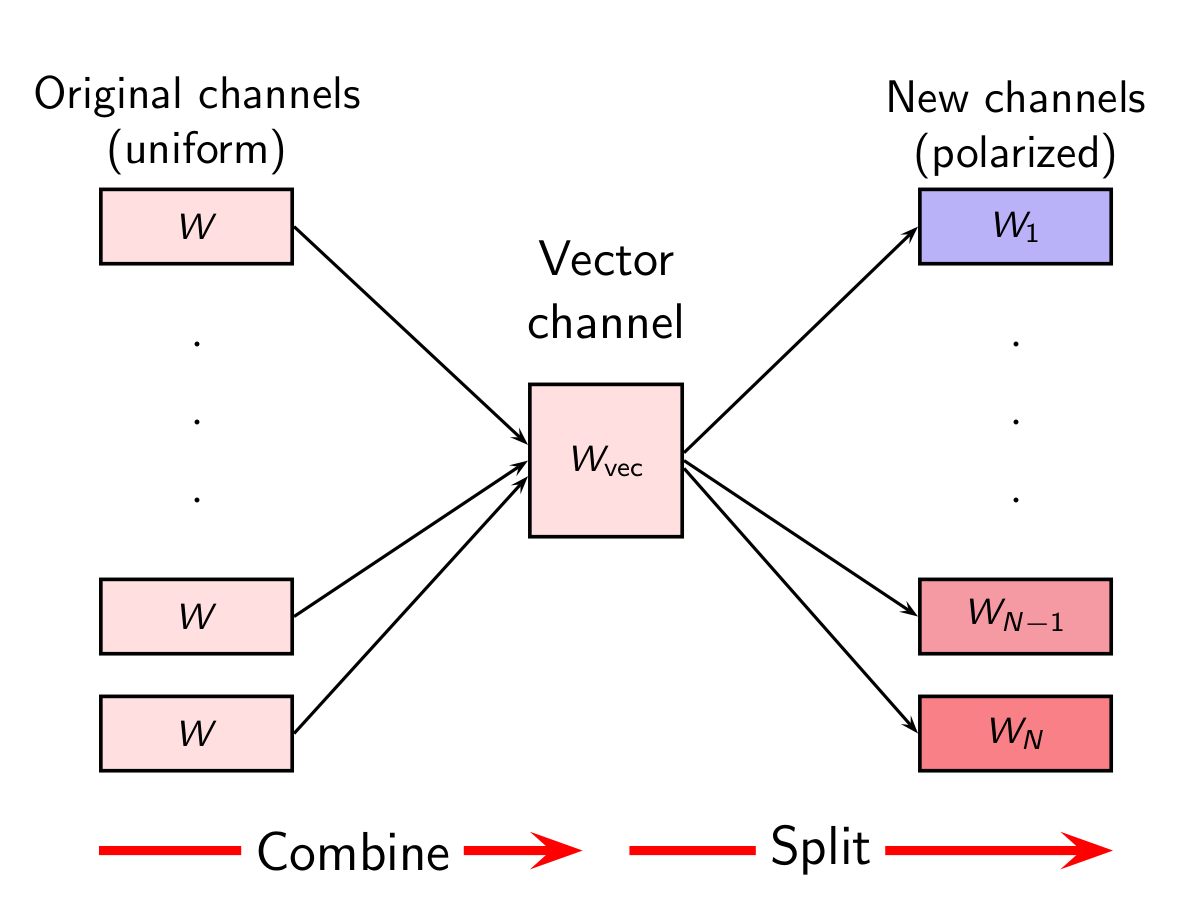
\includegraphics[width=4cm]{./channelcomb.png}
\end{figure}
\end{column}
\begin{column}{0.4\textwidth}
\begin{figure}
\centering
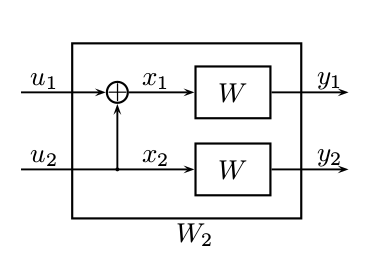
\includegraphics[width=4cm]{./arikanfly.png}
\caption{Transformation butterfly}
\end{figure}
\end{column}
\end{columns}
\end{minipage}
\begin{itemize}
\item $N$ independent copies of a given B-DMC ($W$) are combined and split into a second set of $N$ channels $\{W^{(i)}_N : 1 \leq i \leq N \}$.
\item There symmetric capacity $I(W^{(i)}_N )$ tend towards $0$ or $1$.
\item The channels with Bhattacharya parameter $Z(W^{(i)}_N)=0$ captures the capacity of $W_{vec}$.
\end{itemize}
\end{frame}

%----------------------polar encodedecode
\begin{frame}[label = polarencodedecode]
\frametitle{Brief Introduction to Polar Codes}
\framesubtitle{Encoding and decoding}
\begin{figure}
\centering
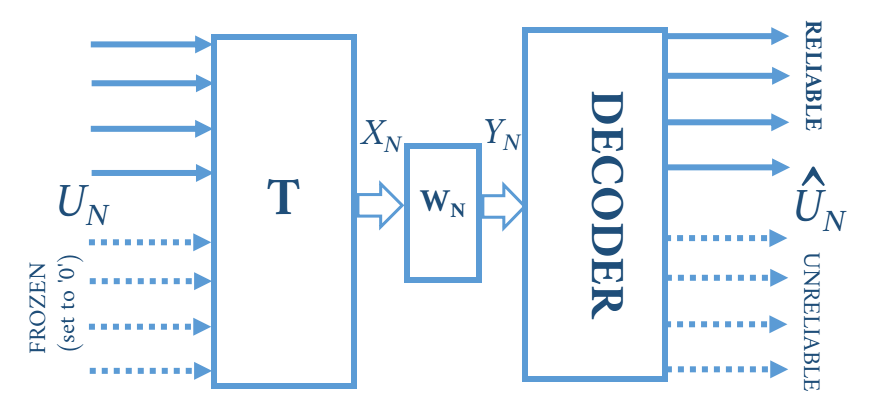
\includegraphics[width=7cm]{./pchschemep.png}
\end{figure}
\begin{itemize}
\item The encoding process\footnote{\tiny {$U_N$ is a uniform message vector, $T$ is a linear transform for the butterfly.}} sends data on transformed channels with $Z(W^{(i)}_N)=0$  (\emph{good channels}) and treats the channels with $Z(W^{(i)}_N)=1$ as \emph{frozen}, sending no useful data on them.
\item For our purpose, we shall be using Succesive Cancellation (SC) decoding.
\end{itemize}
\hypercorner{\hyperlink{polarencode}{\beamerbutton{Encoding}} \hyperlink{polardecode}{\beamerbutton{SC-Decoding}} \hyperlink{polarperformance}{\beamerbutton{Performance}}}
\end{frame}

%----------------------polar slepian
\begin{frame}[label = polarslepian]
\frametitle{Slepian-Wolf compression with Polar Codes}
\begin{figure}
\centering
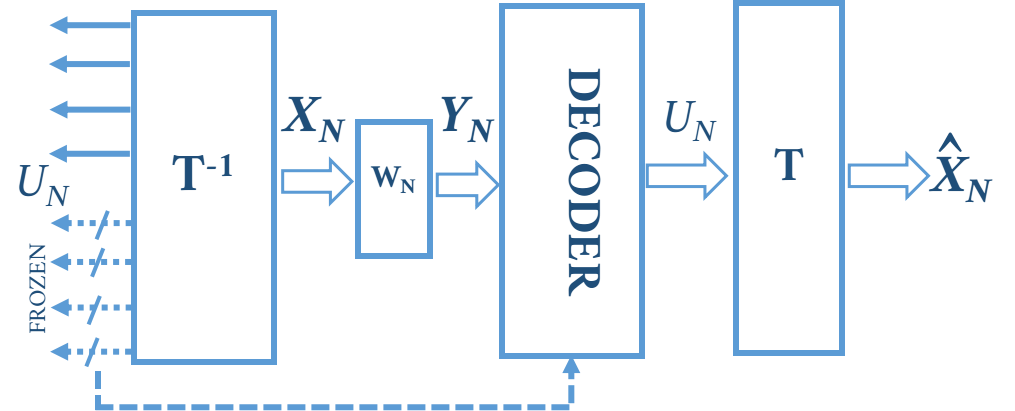
\includegraphics[width=7cm]{./pswschemep.png}
\end{figure}
\begin{itemize}
\item $Y_N$ is a corrupted version of $X_N$ by $N$ BSC(p) channels.
\item The bits that are to be sent for estimation of $X_N$ from $Y_N$ are the frozen bits in $U_N$.  
\item These bits are communicated error free to the SC-decoder. 
\item $H(X_N)-I(W_N)=H(X_N/Y_N)$ bits are sent. 
\end{itemize}
\hypercorner{ \hyperlink{polarswperformance}{\beamerbutton{Performance}}}
\end{frame}
%---------------------Rateless polar codes
\begin{frame}[label = rpc]
\frametitle{Rateless Polar Codes}
\framesubtitle{Rateless code}
\begin{block}{Rateless Code}
A rateless coding scheme transmits incrementally more and more coded bits over an unknown channel until all the information bits are decoded reliably by the receiver.
\end{block}
\begin{itemize}
\item A rateless code is designed for a set of channels and judged for its performance for the entire set.
\item In general rateless code design is based on Hybrid-ARQ techniques and uses code puncturing.
\item Rateless Polar Codes can be constructed using nesting property of Polar Codes for degraded channels.
\end{itemize}
\end{frame}
%---------------------degradedness and nesting
\begin{frame}[label = dgnest]
\frametitle{Rateless Polar Codes}
\framesubtitle{Degraded channels and nesting property}
\begin{columns}
\begin{column}{0.6\textwidth}
\begin{block}{Degraded channels} 
if X\---Y\---Z, and $W_1=P_{Y|X}$, $W_2=P_{Z|X}$ then $W_2 \preceq W_1$.
\end{block}
\begin{itemize}
\item The capacity of $W_2$ is lesser than that of $W_1$. $W_2$ has lesser number of good channels.
\item e.g., $BSC(p_1) \preceq BSC(p_2)$ if $p_1 \geq p_2$.
\end{itemize}
\end{column}
\begin{column}{0.3\textwidth}
\begin{figure}
\centering
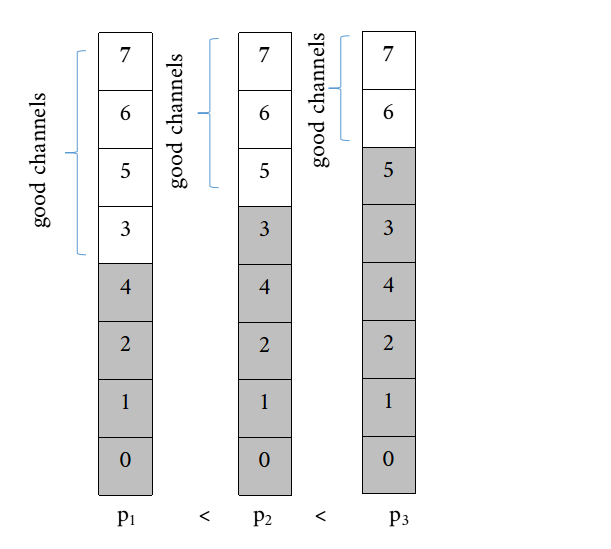
\includegraphics[width=5cm]{./relorder.png}
\end{figure}
\end{column}
\end{columns}
\begin{itemize}
\item The good bit indices of $W_2$ is a subset of the good bit indices of $W_1$.
\item  A more reliable bit-channel is always noiseless if a less reliable bit-channel is noiseless. This leads to \emph{reliability ordering}.
\end{itemize}
\end{frame}
%--------------------------------------IncFrz
\begin{frame}[label = incfrz]
\frametitle{Incremental Freezing}
\framesubtitle{Rateless Polar Code employing reliability ordering}
\begin{figure}
\centering
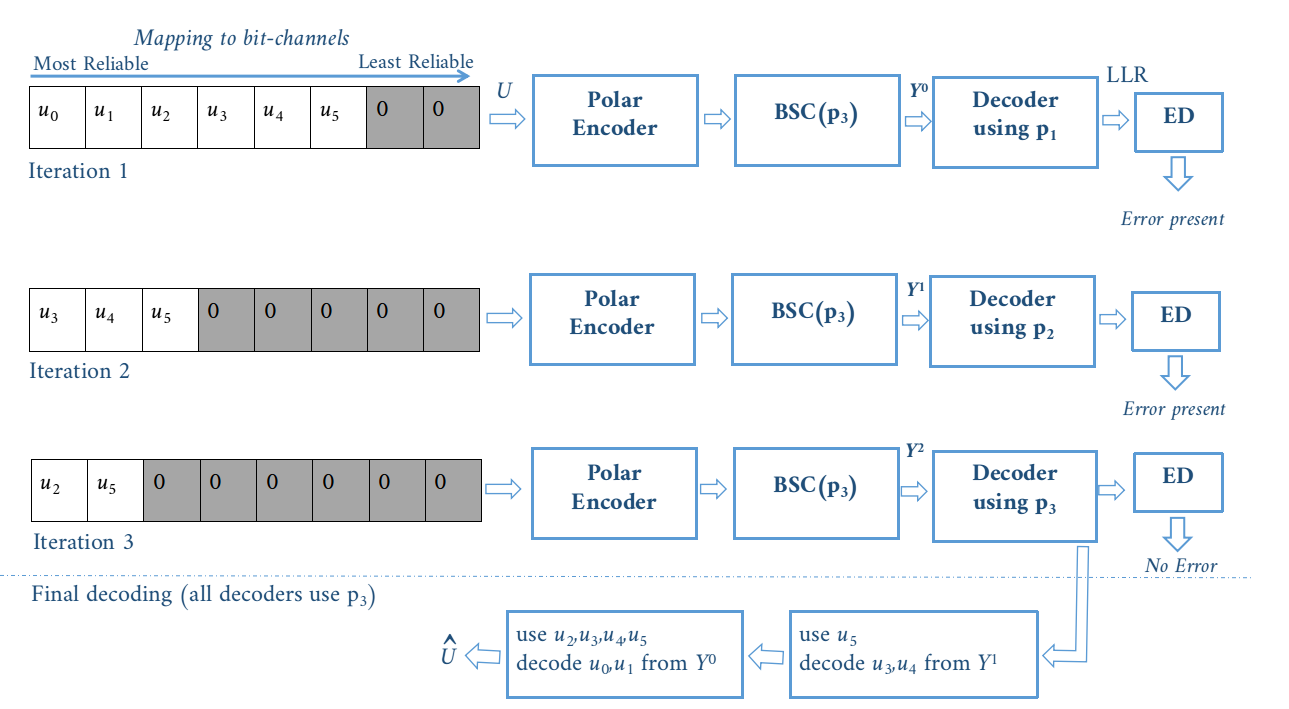
\includegraphics[width=9cm]{./ifp.png}
\end{figure}
\begin{itemize}
\item Initial transmission is done using a high rate Polar Code.
\item If decoding fails then the comparatively lesser reliable channels are retransmitted.  
\end{itemize}
\end{frame}
%-------------------------------incfrz2
\begin{frame}[label = incfrz2]
\frametitle{Incremental Freezing}
\framesubtitle{continued...}
\begin{itemize}
\item Features
\begin{itemize}
\item By decoding the bits from future transmissions they effectively become frozen.
\item This scheme is capacity achieving in the sense that no rate has been wasted.\footnote{\tiny, Figure illustrates the scheme for a set of channels with rates $\{ R_1=6/8, R_2= R_1/2=3/8,R_3= R_1/3=1/4\}$. After the $3^{rd}$ transmission  $u_2$ to $u_{5}$ have been incrementally frozen. The final rate achieved is, $R^*= \frac{6}{8*3}=\frac{1}{4}=R_3 $}
\item A certain number of channels in this scheme is "\emph{always available}" guaranteeing a certain rate in each transmission. 
\item $n$ iterations of the scheme is almost equivalent in performance to a $R/n$ fixed rate Polar Code.
\end{itemize}
\end{itemize}
\end{frame}
%------------------------------HARQ
\begin{frame}[label = HARQ]
\frametitle{Rateless Polar Codes as Hybrid ARQ}
\begin{itemize}
\item Features
\begin{itemize}
\item By decoding the bits from future transmissions they effectively become frozen.
\item This scheme is capacity achieving in the sense that no rate has been wasted.\footnote{\tiny, Figure illustrates the scheme for a set of channels with rates $\{ R_1=6/8, R_2= R_1/2=3/8,R_3= R_1/3=1/4\}$. After the $3^{rd}$ transmission  $u_2$ to $u_{5}$ have been incrementally frozen. The final rate achieved is, $R^*= \frac{6}{8*3}=\frac{1}{4}=R_3 $}
\item A certain number of channels in this scheme is "\emph{always available}" guaranteeing a certain rate in each transmission. 
\item $n$ iterations of the scheme is almost equivalent in performance to a $R/n$ fixed rate Polar Code.
\end{itemize}
\end{itemize}
\hypercorner{ \hyperlink{selrep}{\beamerbutton{Selective Repetition}} \hyperlink{subpol}{\beamerbutton{Subset Polar Codes}} \hyperlink{rbharq}{\beamerbutton{RB-HARQ}}}
\end{frame}
 
%****************************************
\begin{frame}{References}
\begin{enumerate}
\item[(1)] S. Kumar and H. D. Pfister, “Reed-Muller codes achieve
capacity on erasure channels,” 2015, [Online]. Available:
http://arxiv.org/abs/1505.05123v2.
\item[(2)] S. Kudekar, M. Mondelli, E. \c{S}a\c{s}\u{o}glu, and R. Urbanke, “Reed-Muller codes achieve capacity on the binary erasure channel under MAP
decoding,” 2015, [Online]. Available: http://arxiv.org/abs/1505.05831v1.
\item[(3)] {\color{MidnightBlue}$\equiv (1) \cup (2)$} S. Kudekar, S. Kumar, M. Mondelli, H. D. Pfister, E. \c{S}a\c{s}\u{o}glu, and R. Urbanke, “Reed-Muller codes achieve
capacity on erasure channels,” 2016, [Online]. Available:
http://arxiv.org/abs/1601.04689v1.
\end{enumerate}
\end{frame}

\begin{frame}
\frametitle{}
\begin{figure}[!htb]
\begin{center}

\includegraphics[scale=0.35]{./figures/questions.jpg}
\end{center}
\end{figure}
\begin{block}{}
\centering
Thank You!
\end{block}
\end{frame}

%============================Backup slides
\section{Appendix}
%---rsync
\begin{frame}[label = rsync]
\frametitle{The r-sync protocol}
\hyperlink{rsynccomp}{\beamerbutton{back}}
\end{frame}
%---polar encoding
\begin{frame}[label = polarencode]
\frametitle{Polar Encoding}
\hyperlink{polarencodedecode}{\beamerbutton{back}}
\end{frame}
%-----polar decode
\begin{frame}[label = polardecode]
\frametitle{Succesive Cancellation Decoding}
\hyperlink{polarencodedecode}{\beamerbutton{back}}
\end{frame}
%-----------------------polar performance
\begin{frame}[label = polarperformance]
\frametitle{Performance of Polar Codes}
\begin{figure}
\centering
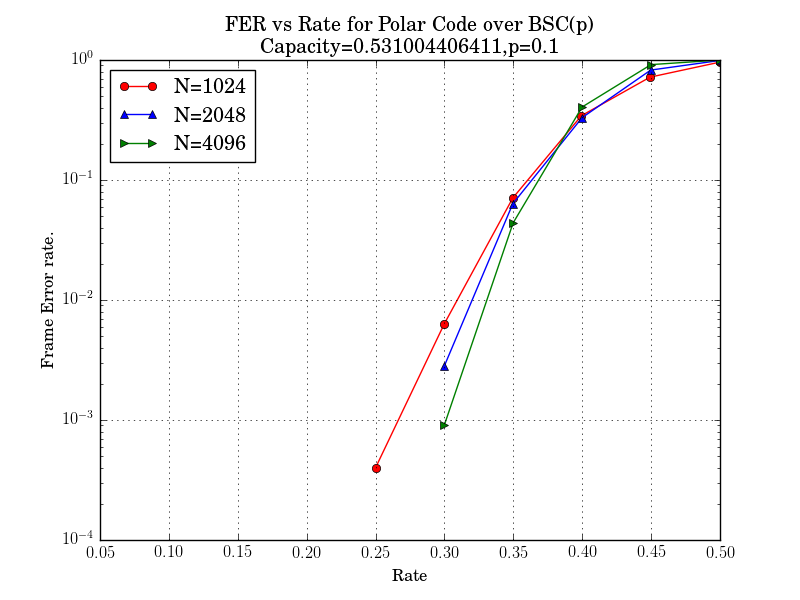
\includegraphics[width=9cm]{./fer.png}
\end{figure}
\hyperback{\hyperlink{polarencodedecode}{\beamerbutton{back}}}
\end{frame}
%---------------------polarsw
\begin{frame}[label = polarswperformance]
\frametitle{Performance of SW compression Polar Codes}
\begin{figure}
\centering
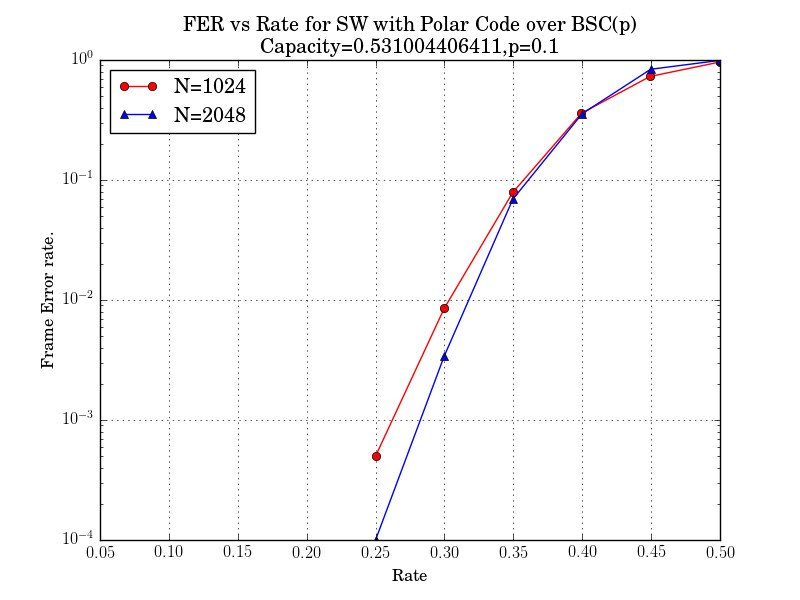
\includegraphics[width=9cm]{./swfer.png}
\end{figure}
\hyperback{\hyperlink{polarslepian}{\beamerbutton{back}}}
\end{frame}
%---------------------selective repetition
\begin{frame}[label = selrep]
\frametitle{Selective Repetition H-ARQ for polar codes}
\begin{columns}
\begin{column}{0.4\textwidth}
\begin{itemize}
\item Initially, an information block of $K$ bits is fed into a polar encoder.
\item The output codeword of $N_0$ bits is punctured into $N_1$
bits and sent over the channel.
\end{itemize}
\end{column}
\begin{column}{0.5\textwidth}
\begin{figure}
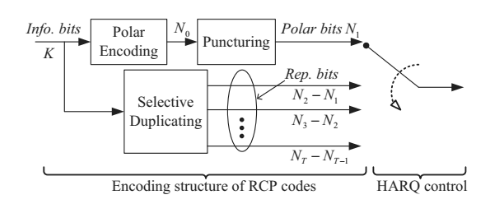
\includegraphics[width=6cm]{./selrepharq.png}
\end{figure}
\end{column}
\end{columns}
\begin{itemize}
\item {Retransmission process}
\begin{itemize}
\item On decoding failure reciever sends a NACK.
\item $N_2-N_1$ of the information bits are retransmitted. 
\item The receiver tries to perform decoding with all the $N_2$ received
bits.
\item This process continues until the transmitter
receives an ACK 
\end{itemize}
\end{itemize}
\hyperback{\hyperlink{HARQ}{\beamerbutton{back}}}

\tiny The retransmitted bits (RV) are chosen one at a time as the most unreliable of the $K$ bits transmitted, reliability is calculated after choosing one bit and the process is iterated.
\end{frame}
%---------------------subset polar
\begin{frame}[label = subpol]
\frametitle{Subset Polar Codes}
\begin{itemize}
\item A Subset Polar Code can be created by greedily puncturing a low-rate mother code without re-optimizing the information bits.
\item The scheme uses equivalent Subset Polar Codes as RV.
\item This has the better performance compared to other HARQ methods.
\end{itemize}
\hyperback{\hyperlink{HARQ}{\beamerbutton{back}}}
\end{frame}
%---------------------RB-HARQ
\begin{frame}[label = rbharq]
\frametitle{Reliability based HARQ}
Reliability based HARQ technique (RBHARQ) , eliminates the use of CRC by approximating bit and word error probability from likelihood ratios (LLR).   The bit error probability for the $k^{th}$ bit can be estimated from LLR ($\tilde{u}_k$) as,
\begin{equation}\label{eq:errorllr}
P_{b,k}=P(\hat{u_k} \neq u_k) = \frac{1}{1+e^{|\tilde{u}_k|}}
\end{equation}
then word error probability becomes, 
\begin{equation}
P_w=1-e^{log\bar{P}_w}
\end{equation}
where, $$log\bar{P}_w=log\prod_{k=1}^K (1- P_{b,k})$$ 
If the word error probability does not meet the requirements the bits with higher bit error probability may be retransmitted. This increases throughput, particularly evident in case of short packet lengths.
\hyperback{\hyperlink{HARQ}{\beamerbutton{back}}}
\end{frame}

\end{document}

